% \documentclass[sigconf,anonymous,review,timestamp]{acmart}
\documentclass[sigconf]{acmart}

%% Rights management information.  This information is sent to you
%% when you complete the rights form.  These commands have SAMPLE
%% values in them; it is your responsibility as an author to replace
%% the commands and values with those provided to you when you
%% complete the rights form.
\setcopyright{acmcopyright}
\copyrightyear{2023}
\acmYear{2023}
\acmDOI{XXXXXXX.XXXXXXX}

%% These commands are for a PROCEEDINGS abstract or paper.
\acmConference[Conference acronym 'XX]{Conference title}{January 01--02,
  1900}{Someplace, NY}
\acmPrice{15.00}
\acmISBN{978-1-4503-XXXX-X/18/06}

%%
%% Submission ID.
%% Use this when submitting an article to a sponsored event. You'll
%% receive a unique submission ID from the organizers of the event,
%% and this ID should be used as the parameter to this command.
\acmSubmissionID{123-A56-BU3}

%%
%% The majority of ACM publications use numbered citations and
%% references.  The command \citestyle{authoryear} switches to the
%% "author year" style.
%%
%% If you are preparing content for an event
%% sponsored by ACM SIGGRAPH, you must use the "author year" style of
%% citations and references.
%% Uncommenting
%% the next command will enable that style.
\citestyle{acmauthoryear}

%%%%%%%%%%%%%%%%%%%%%%%%%%%%%%%%%%%%%%%%%%%%%%%%%%%%%%%%%%%%%%%%%%%%%%%%%%%%%%%%
%% TODO 20221010 temp
\usepackage{todonotes}
%%%%%%%%%%%%%%%%%%%%%%%%%%%%%%%%%%%%%%%%%%%%%%%%%%%%%%%%%%%%%%%%%%%%%%%%%%%%%%%%

\begin{document}

\title{Coevolution of Camouflage}

%% Author
\author{Craig Reynolds}
\email{cwr@red3d.com}
\orcid{0000-0001-8203-712X}
\affiliation{%
  \institution{unaffiliated researcher}
  \country{USA}
}

\renewcommand{\shortauthors}{Craig Reynolds}

\begin{abstract}
  [... super preliminary ... an abstract model of the evolution of camouflage in nature through adversarial interaction between predator and prey ... model contains representation of populations of predator and prey ...]
  [... produces camouflage textures for given backgrounds (typically photos of the real world) based on mutual conflict between predators and prey]
\end{abstract}

%%
%% Generate your CCSCML using http://dl.acm.org/ccs.cfm.
%%
\begin{CCSXML}
<ccs2012>
   <concept>
       <concept_id>10010147.10010341.10010349.10011810</concept_id>
       <concept_desc>Computing methodologies~Artificial life</concept_desc>
       <concept_significance>500</concept_significance>
       </concept>
   <concept>
       <concept_id>10010147.10010371.10010382.10010384</concept_id>
       <concept_desc>Computing methodologies~Texturing</concept_desc>
       <concept_significance>500</concept_significance>
       </concept>
   <concept>
       <concept_id>10010147.10010178.10010224</concept_id>
       <concept_desc>Computing methodologies~Computer vision</concept_desc>
       <concept_significance>500</concept_significance>
       </concept>
    
    <concept>
        <concept_id>10010147.10010257.10010293.10011809.10011813</concept_id>
        <concept_desc>Computing methodologies~Genetic programming</concept_desc>
        <concept_significance>500</concept_significance>
    </concept>
 </ccs2012>
\end{CCSXML}

\ccsdesc[500]{Computing methodologies~Artificial life}
\ccsdesc[500]{Computing methodologies~Texturing}
\ccsdesc[500]{Computing methodologies~Computer vision}
\ccsdesc[500]{Computing methodologies~Genetic programming}

%% Keywords
\keywords{camouflage, coevolution, nature, biology, predator, prey, vision, texture synthesis}

%% Teaser figure that appears on the top of the article.
\begin{teaserfigure}
    %% TODO note: use images without the “predator prediction crosshairs”.
    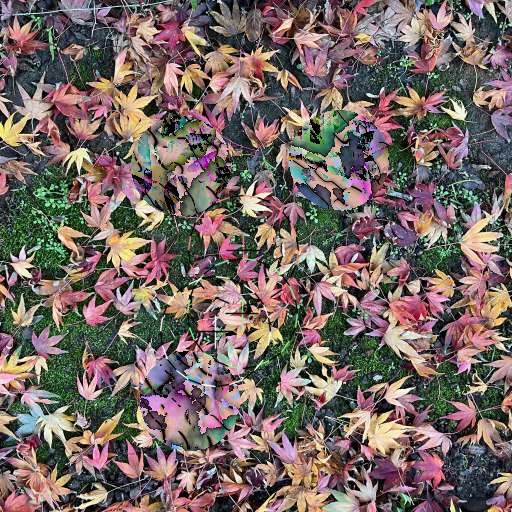
\includegraphics[scale=0.24]{images/20220918_step_7372.png}
    \hfill
    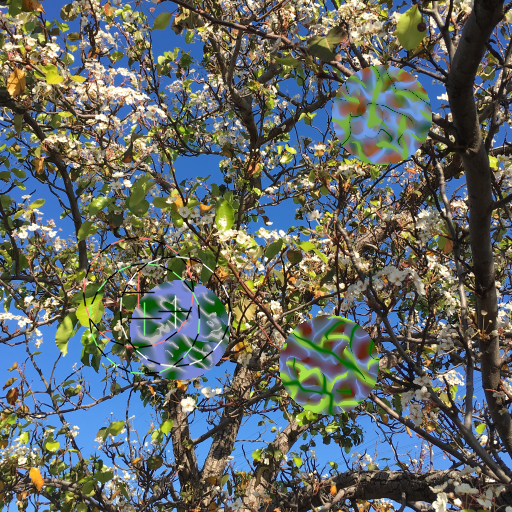
\includegraphics[scale=0.24]{images/20220926_step_6143.png}
    \hfill
    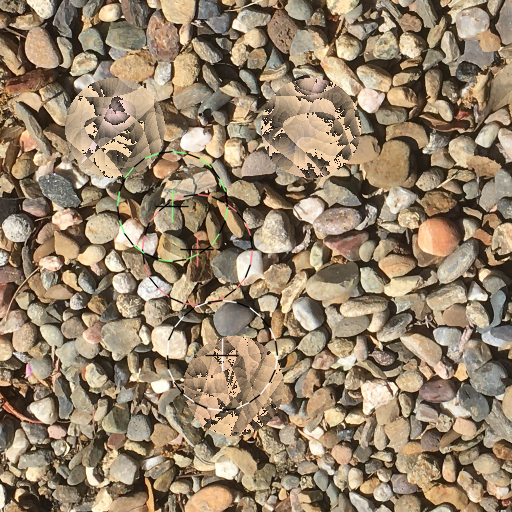
\includegraphics[scale=0.24]{images/20221003_step_3667.png}
    \hfill
    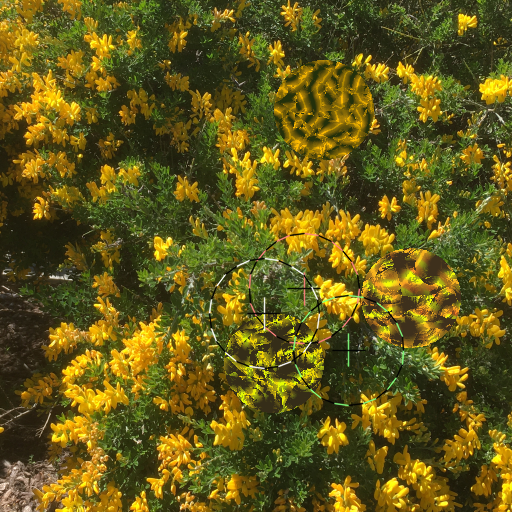
\includegraphics[scale=0.24]{images/20220930_step_6093.png}
    \caption{Photographs of natural textures, each overlaid with three camouflaged \textit{prey}. The prey are randomly placed 2D disks, each with its own evolved camouflage texture. [QQQ replace stand-in images]}
    \Description{Examples of camouflage textures produced by the simulation.}
    \label{fig:teaser}
    % \vspace{5mm} %5mm vertical space
    \vspace{3mm} % 3mm vertical space
\end{teaserfigure}

%% I guess this lays out the single column “top matter” defined above.
\maketitle

\section{Introduction}
This work aims to create a simplified and abstract 2d simulation model of the evolution of camouflage textures in nature. These camouflage patterns emerge in the interaction, the coevolution, of a population of \textit{prey} each with a candidate texture and a population of \textit{predators} each with a learned visual detector. The input to the simulation is a set of photos of a background environment. The prey evolve to be \textit{cryptic} — hard to see — against the background images. The predators evolve and learn to hunt the prey by locating their position within the environment.
\par
Computational models of complex biological systems have several benefits. Constructing them, getting them to work as seen in nature, helps crystallize our thinking about natural phenomenon. Computational models also allow experimentation \textit{in silico} to help characterize this complex natural systems.
\par
[... introduction ... following the approach of \citet{Reynolds2011} a population of prey, each with a synthetic camouflage texture, are evolved against negative selection by a predator which prefers the most conspicuous prey against a given background. ...]
\begin{figure*}
    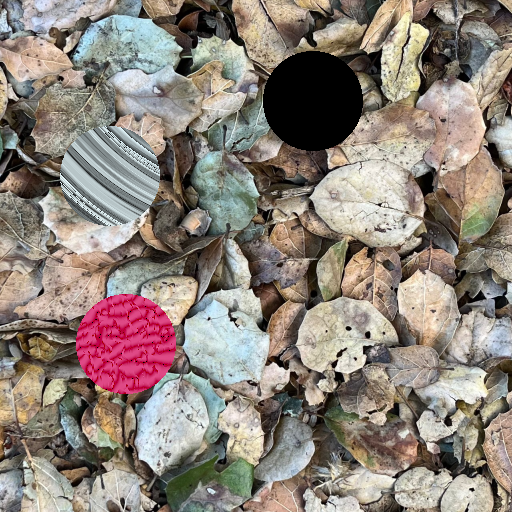
\includegraphics[scale=0.16]{images/20221016_step_969.png}
    \hfill
    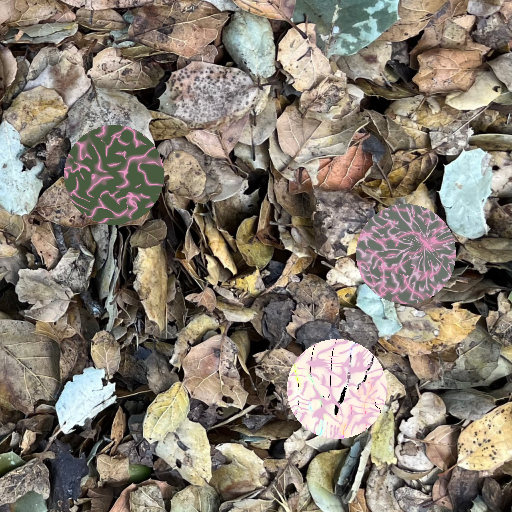
\includegraphics[scale=0.16]{images/20221016_step_1710.png}
    \hfill
    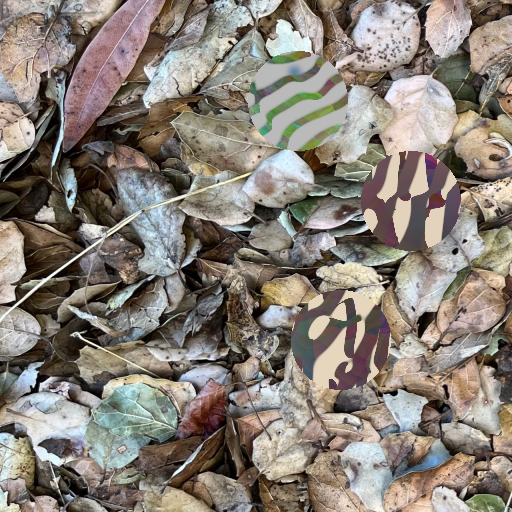
\includegraphics[scale=0.16]{images/20221016_step_2368.png}
    \hfill
    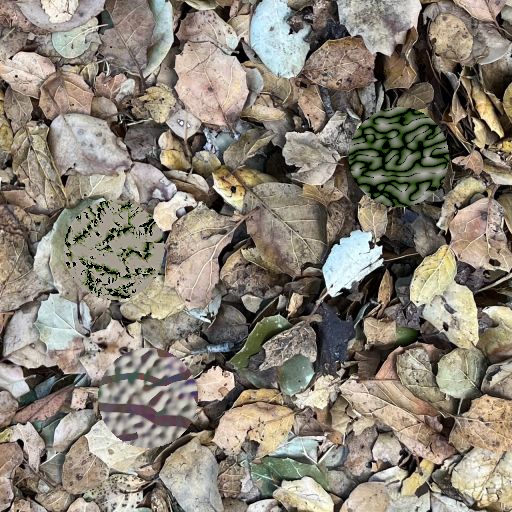
\includegraphics[scale=0.16]{images/20221016_step_3420.png}
    \hfill
    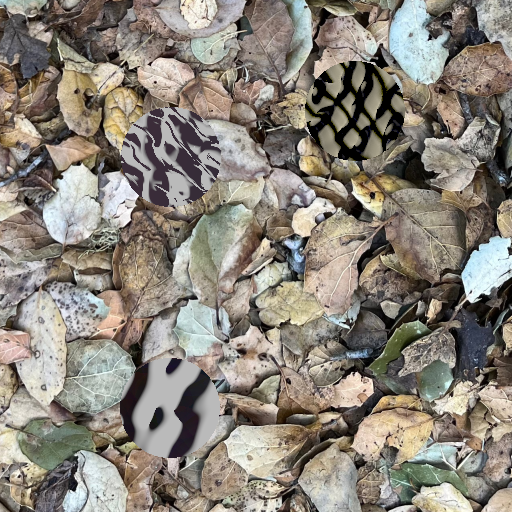
\includegraphics[scale=0.16]{images/20221016_step_4864.png}
    \hfill
    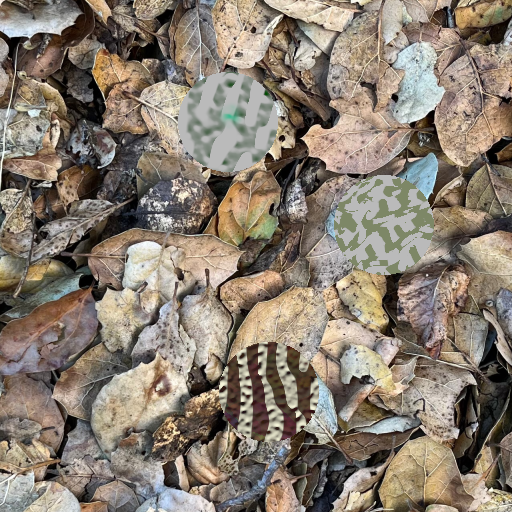
\includegraphics[scale=0.16]{images/20221016_step_5564.png}
    \caption{Evolution of the prey population over simulation time}
    \Description{Sequence of images showing evolution of prey population over simulation time.}
    \label{fig:time_sequence}
    \vspace{5mm} %5mm vertical space
\end{figure*}

\section{Related work}
[... \textbf{closely related work:} 
[... \cite{harrington_coevolution_2014} ...]
and
GANmouflage \cite{guo_ganmouflage_2022} and \cite{owens_camouflaging_2014} ...] 
\par
[... TexSyn \textbf{[OK to mention name?]} is based on the “strongly typed” variant of Genetic Programming known as STGP \cite{montana_strongly_1995}, one of several grammar-based GP variants \cite{Mckay_2010}. ...]


\section{Simulation and competition}
\subsection{Random topics QQQ}
This camouflage simulation is based on two adversarial \textbf{populations}: one of \textbf{predators} and one of \textbf{prey}. Individual prey and predators compete with their own kind for survival within their own population. Predators must \textbf{hunt} successfully to survive. Prey survive if inconspicuous (“cryptic”) enough to avoid being found and eaten. A prey hunted and eaten — or a predator perished from hunger — is removed from its population. It is replaced by an \textbf{offspring} of parents from the surviving population.
\par
Predators define the fitness of prey: being easy to spot is bad, blending in is good. Similarly prey define the fitness of predators: being fooled by camouflage is bad, spotting cryptic prey is good. From this adversarial interaction, the two populations \textbf{coevolve}. If one side has some sort of flaw, the other side has a motivation to exploit it. As a result both sides tend to improve over simulation time.
\par
Initial random prey have coloration likely to contrast with the background. Initial predators have a “pre-trained” ability to find conspicuous objects which may allow them to hunt the initial un-camouflaged prey.
\par
[... relative fitness ...] and [... negative selection ...]
\par
[... tournaments relative fitness in game-like competition ...]

\section{Texture Synthesis}
Textures are represented in this simulation as trees of procedural texture operators. These correspond directly to nested expressions in a typical programming language. \textbf{TexSyn} is a simple domain specific language for describing textures.
\par
The details of TexSyn are not central to understanding this camouflage model. A quick overview is given here. TexSyn is library, an API, with many \textbf{operators} each of which return a \textbf{Texture}. Almost all of them also take Textures as input parameters, along with simple values like colors, 2d vectors, and floating point numbers. Writing nested functional expressions of operators corresponds to trees of operator instances.
\par
These TexSyn style textures are represented as operators, trees, and parameters. They do not store pixel data, providing instead a function to sample the textures color at an arbitrary floating point xy location. This is similar to fragment shaders for GPU and the Pixel Stream Editor functions in \cite{perlin_image_1985}.
\par
%%
%% mention here, or in Related Work?:
%%     Karl Sims. 1991. Artificial Evolution for Computer Graphics.
%%     Computer Graphics, 25(4):319–328.
%%     https://www.karlsims.com/papers/siggraph91.html  [ACM DL DOI?]
%%
\begin{figure}
\centering
% \missingfigure is from todonotes
\missingfigure[figwidth=\linewidth*0.5,figcolor=white]{}
\caption{TexSyn example}
\end{figure}

\section{Limitations}
[... no objective measure of camouflage effectiveness ...]
\par
[... all results are hand selected, “cherry picked” ...] 
\par
[... cite that fast growing literature on “camouflaged object detection” ...]
\par
[... propose a crowd sourced user study of camouflage quality ... could be based on time to find ... like the interactive web games of \href{https://www.visual-ecology.com/2020/10/06/martin-stevens/}{Martin Stevens} nuthatch egg? ...] 
\par
[... in email to Ken I wrote: \textit{The aspect of my project I'm unsure how to approach is lack of rigor. My evaluations are all subjective. It comes down to “we can see that the effectiveness of the camouflage clearly increases during the simulation.”}]
\par
[... inherently 2d ...]
\par
[... texture synthesis lacks genetic or biological plausibility ...]


%% Acknowledgements
\begin{acks}
[... Many thanks to all who helped me with this work: my supportive family, Andrew Glassner for teaching me everything I know about deep learning, Ken Perlin for, lots, but especially [An Image Synthesizer?] Pat Hanrahan for helpful career advice (“just do the research”). ...]
\par
[maybe just names (roughly backward in time): 
Ken Perlin,
Andrew Glassner,
Pat Hanrahan,
Karl Sims,
John Koza,
Richard Dawkins,
Witkin/Kass/Turk,
Peter Angeline,
Jordan Pollack.
and of course, Alan Turing. [too weird/maudlin? QQQ]
]
\end{acks}


%% Bibliography.
\bibliographystyle{ACM-Reference-Format}
\bibliography{coc.bib}


%% Appendix
\appendix

\section{Additional Section}
Text

% Note (from https://s2022.siggraph.org/technical-papers-submissions-faq/): 
% The Conference Paper track encourages submissions for high-quality, 
% ground-breaking research that fits within a strict 7-page limit (plus 
% additional pages for references), and may be more appropriate for
% research that is less-polished but still potentially-impactful. Journal 
% papers do not have a page limit, and may include more thorough experiments
% and derivations within the main paper. 

\end{document}
